\documentclass[11pt,a4paper]{article}

\usepackage[T1]{fontenc}
\usepackage[utf8]{inputenc}
\usepackage[frenchb]{babel}

\usepackage{fancyhdr} % headers
\usepackage[usenames,dvipsnames]{color} % colors
\usepackage{graphicx} % images
\usepackage{listings} % source code
\usepackage{titling} % meta-infos
\usepackage{courier} % courier font
\usepackage{fullpage} % full page layout
\usepackage{titlesec} % title customization
\usepackage{parskip} % paragraphs spacing
\usepackage{amsmath}
\usepackage{tikz}
\usepackage{siunitx}
%\usepackage{showframe} % layout debug

\usepackage{float}
\restylefloat{figure}

\topmargin -10mm
\headsep 5mm
\headheight 10mm

\linespread{1.1}
\renewcommand{\arraystretch}{1.3}

\setlength\parindent{0pt}
\setlength{\unitlength}{1cm}
\setlength{\droptitle}{-1.6cm}

\pagestyle{fancy}
\fancyhf{}
\cfoot{\thepage}

\def \doccourse { ARO2-C }
\def \doctitle {Labo : Microarchitecture EXECUTE et MEMORY}
\author{Bastien Clément Christophe Peretti \\
  Professeur: Michel Starkier}

\renewcommand{\thesection}{Partie \arabic{section} :}
\renewcommand{\thesubsection}{\arabic{section}.\arabic{subsection}}

\rhead{\theauthor \\ \today}
\lhead{\doccourse \\ \doctitle }
\title{{\normalsize \doccourse} \\ \doctitle }

\begin{document}

\maketitle
\vspace{1em}

\section{EXECUTE}

Les objectifs de cette première partie sont de réaliser une partie EXECUTE simplifiée d'un processeur sur logisim, en ajoutant les opérations arithmétiques et logiques, ainsi que les shifts. Les blocs FETCH et DECODE nous sont fournis, ainsi qu'un programme à exécuter.

\subsection{Analyse du bloc Decode}

Afin de pouvoir exécuter correctement les instructions dans le bloc $Execute$, il faut tout d'abord que nous analysions comment sont traitées les instructions dans le bloc $Decode$. Ce bloc nous a été fournis pour ce laboratoire et est donc plus complet que celui que nous avions réalisé lors du précédent labo. Le bloc $Decode$ fournit est constitué de deux parties, le $Data\ Splitter$ et le $Control\ Unit$.

Le $Data Splitter$ nous permet d'extraire les différentes valeurs de l'instruction, comme les numéros de registre (source et destination), et les valeurs immédiates. C'est ce bloc qui transmettra les numéros de registre à la banque de registre d'une part, et les valeurs immédiates au bloc $Execute$ d'autre part.

Le $Control\ Unit$ quant à lui, analyse la commande à proprement parler, et active ou désactive les différents bit de sélection de tous les mux et registres afin que le bloc $Execute$ travaille correctement. Avec toutes ces valeurs, il les met en série et en fait un bus, l' $execute\_control\_bus$ qu'il transmet au bloc $Execute$.

Ci-dessous, le chronogramme généré à partir du code fournit:
\begin{tabbing}
$mov\ \ $\=$ r0,\ \#5$ \\
$mov$\>$r1,\ r0$ \\
$add$\>$r4,\ r1,\ \#7$ \\
$add$\>$r5,\ r4,\ r0$ \\
$and$\>$r4,\ r5$ \\
$lsl$\>$r2,\ r5,\ \#3$ \\
$sub$\>$r0,\ r4,\ r2$ \\
\end{tabbing}


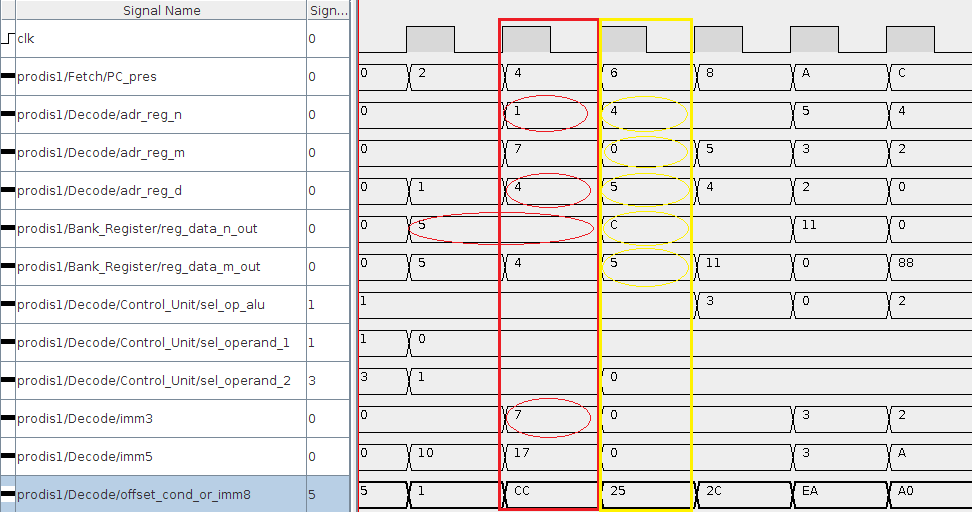
\includegraphics[width=15.8cm]{img_Chronogram.png}

Faisons une analyse de l'instruction $add\ \ r4,\ r1,\ \#7$, encadrée en rouge. Pour une instruction, il n'y a pas toujours toutes les valeurs qui sont utiles. Ici, nous avons un registre de destination ainsi qu'un registre source et une valeur immédiate.

Pour l'instruction $add$, la valeur immédiate est sur 3 bits et c'est sans surprise que nous voyons un 7 à cette ligne. De même pour les deux registres, r4 est bien le registre de destination et r1 est le registre source (n). L'instruction fait donc une addition de r1 avec 7 et met le résultat dans r4. Le registre r1 avait été auparavant copié de r0, qui contenait la valeur 5.

Sur le chronogramme, nous voyons, toujours en rouge, la valeur 5 qui est en sortie de la banque de registre et qui est donc le contenu de r1. Les autres valeurs comme imm5 ou adr\_reg\_m ne sont pas utiles pour cette instruction.

L'instruction suivante, $add\ \ r5,\ r4,\ r0$ est encadrée en jaune. Nous pouvons voir que ce ne sont pas les mêmes valeurs qui sont nécessaires pour cette instruction. En effet, il n'y a pas de valeur immédiate mais il y a deux registres source. Nous additionnons r4 et r0 et mettons le résultat dans r5. 

Le registre r4 valait 12 (C), car c'était le résultat de l'opération précédente. Le registre r0 quant à lui, vaut toujours 5 depuis le début. Ces deux valeurs sont visibles aux lignes $reg\_data\_n\_out$ et $reg\_data\_m\_out$. Les autres valeurs entourées sont les numéros des deux registres source et celui du registre de destination.

\newpage
\subsection{Réalisation du bloc Execute}

Maintenant que nous savons précisément les valeurs que nous envoie le bloc Decode, nous pouvons réaliser le bloc Execute. Comme son nom l'indique, c'est ce bloc qui effectue les opérations arithmétiques et logiques du processeur. Il est constitué de trois parties: 

La première effectue quelques opérations sur les entrées afin de pouvoir effectuer les opérations correctement. La deuxième consiste en une série de shifts (arithmétique, logique et rotation). Et la troisième partie est l'ALU (opérations arithmétiques et logiques).

\begin{center}
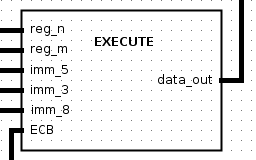
\includegraphics[width=5cm]{img_bloc_execute.png}
\end{center}

Le Bloc Execute prend en entrée les différentes valeurs qui viennent du bloc Decode ($imm\_3$, $imm\_5$, $imm\_8$ et $execute\_control\_bus$) et de la banque de registre ($reg\_n$, $reg\_m$), et livre le résultat qui devra être stocké dans un registre ($data\_out$).

Pour l'étape 2, il nous était demandé de réaliser le circuit nécessaire à la réalisation du programme fournit. Toutefois, ayant la liste de toutes les opérations présente dans l'$execute\_control\_bus$, nous avons directement réalisé les circuits permettant d'effectuer toutes les opérations lors de cette étape.

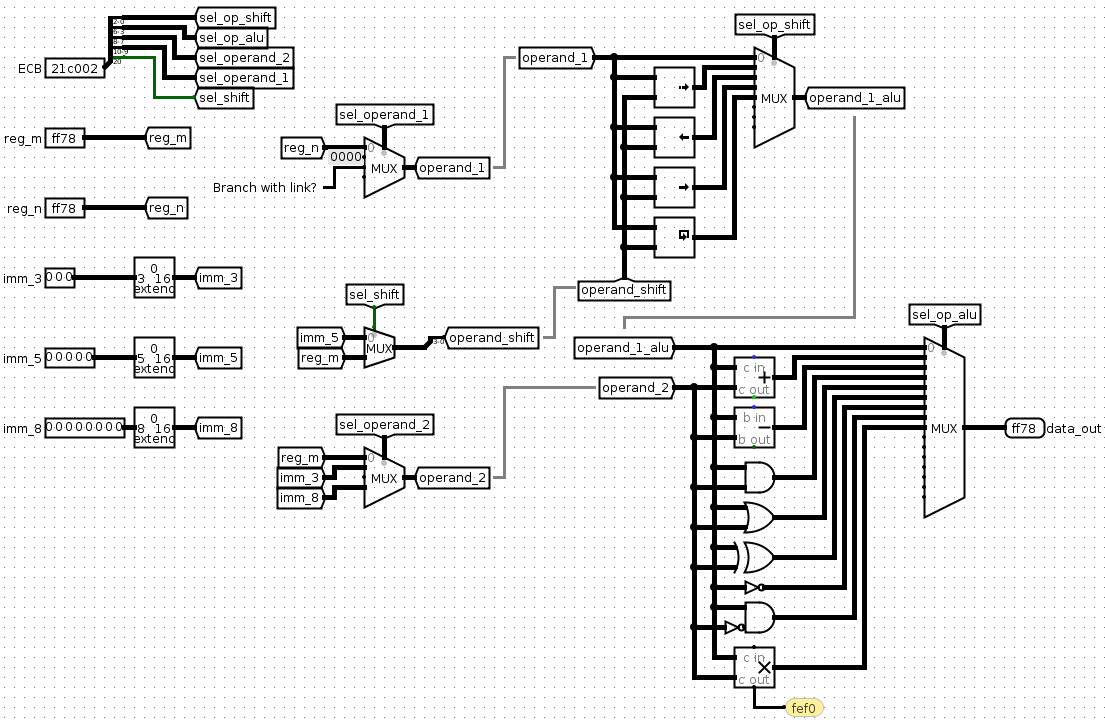
\includegraphics[width=15.3cm]{img_execute.png}

Nous voyons sur ce schéma, les trois parties composants le bloc: Réception des valeurs à gauche, Shifts en haut à droite et ALU en bas à droite.

Ce bloc n'est pas difficile à réaliser. Il ne fait qu'appliquer ce que le bloc Decode lui dit de faire. Pour commencer, il extrait les différents bits de sélection de l'$execute\_control\_bus$ (ECB). Ces bits contrôlent les différents mux du bloc. Dans sa première partie, le bloc étend aussi les valeurs immédiates sur 16 bits, afin d'effectuer les opérations sur un nombre de bits fixe.

Dans la partie Shift, les quatre différents shifts (arithmétique à droite, logique à gauche, logique à droite et rotation à droite), sont mis en parallèle dans un mux contrôlé par le $sel\_op\_shift$ extrait de l'ECB. Une entrée du mux est aussi un bypass, dans le cas où l'on ne souhaite pas effectuer de shift sur l'opérande 1.

Concernant l'ALU, il s'agit de la même configuration que pour les shifts: Les différentes opérations sont mises dans un mux contrôlé par le $sel\_op\_alu$. De façon identique à la partie shift, il y a aussi un bypass de l'opérande 1 dans l'ALU, au cas où l'on ne souhaiterait effectuer aucune opération dans l'ALU, mais uniquement un shift.

Ci-dessous, le chronogramme représentant un programme écrit pour tester toutes les opérations du bloc Execute, y compris la multiplication qui fonctionne parfaitement. Le programme se trouve en annexe.

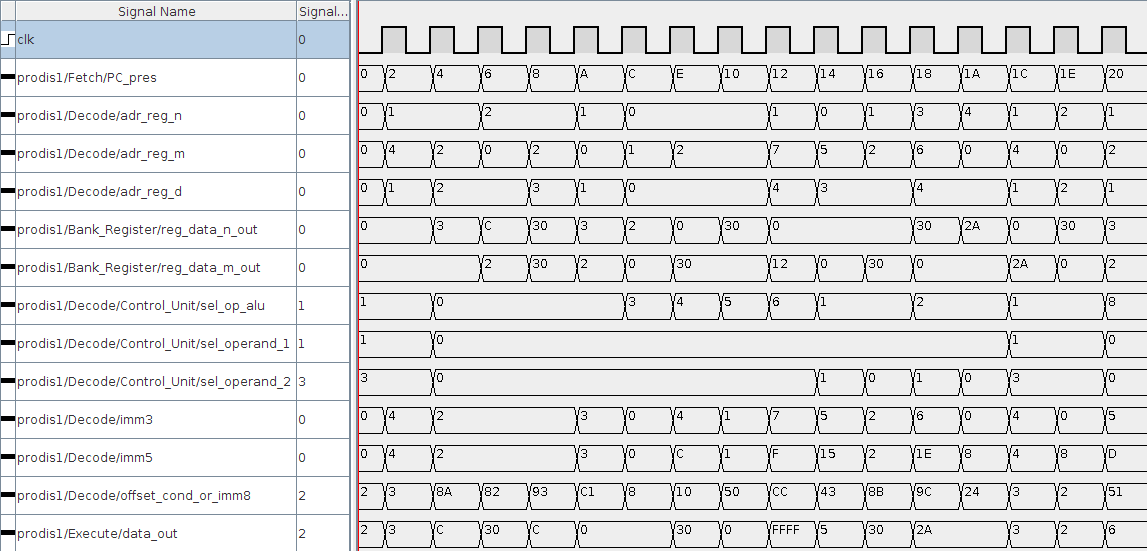
\includegraphics[width=15.8cm]{img_chrono2.png}

\section{MEMORY}

Les objectifs de cette seconde partie du laboratoire sont de comprendre et démonter la partie MEMORY ACCESS du processeur Prodis (fournit), ainsi que comprendre le fonctionnement d'une pile en mémoire. Pour cette partie nous recevons un bloc FETCH du processeur PRODIS ainsi qu'un programme à exécuter.

\newpage
\subsection{Lecture et écriture dans la mémoire}

Dans cette partie du laboratoire, nous utilisons enfin une mémoire afin de stocker des données. En effet, jusqu'à présent, seuls les registres étaient utilisés pour traiter des données. Le nombre de registres étant très limités, il est très utile de pouvoir avoir une mémoire séparée afin de pouvoir enregistrer des données et les traiter plus tard. 

Ayant une architecture Harvard, notre mémoire pour les données est séparée de la mémoire des instructions. De plus, cette mémoire est divisée en deux blocs pouvant contenir des données 8 bits.

Notre premier programme consiste à écrire les valeurs 0x1234 et 0x2468 aux adresses 0x0004 et 0x0006.

Pour charger une donnée 16 bits en mémoire, nous chargeons une valeur immédiate dans un registre $(\#18 = 0x12)$, suivi d'un $shift$, et combiné avec un $or$, nous obtenons une valeur 16 bits.

\begin{tabbing}
$mov\ \ $\=$r0,\ \#18$ \\
$lsl$\>$r0,\ r0,\ \#8$ \\
$mov$\>$r0,\ \#52$ \\
$orr$\>$r0,\ r1$ \\
$mov$\>$r2,\ \#4$ \\
$strh$\>$r0,\ \lbrack r2,\#0 \rbrack$ \\
\end{tabbing}

Une fois ces instructions effectuées, nous pouvons voir que notre valeur 0x1234 a été partagée en deux groupes de 8 bits chacuns, et mis séparément en mémoire, soit 0x12 dans la mémoire $Mem\_high$ et 0x34 dans la mémoire $Mem\_low$.

Nous avons ensuite complété le programme (voir en annexe) afin de déplacer ces valeurs à d'autres adresses dans la mémoire. Il faut donc lire ces valeurs grâce à l'instruction: 

$ldrb\ r3,\ \lbrack r2,\#0\rbrack $

Cette commande va charger dans le registre r3, la valeur (8 bits) présente en mémoire à l'adresse contenue dans r2, avec un offset de 0. Nous remarquons très vite que cette valeur n'est pas 0x12 comme on pourrait le croire, mais bien 0x34 qui était dans la mémoire $Mem\_low$. C'est seulement lorsque nous effectuons la même instruction avec un offset de 1 que nous obtenons notre valeur 0x12. On peut donc en déduire que notre processeur Prodis est $little\ endian$.

\newpage
Voici le chronogramme complet de cette partie:

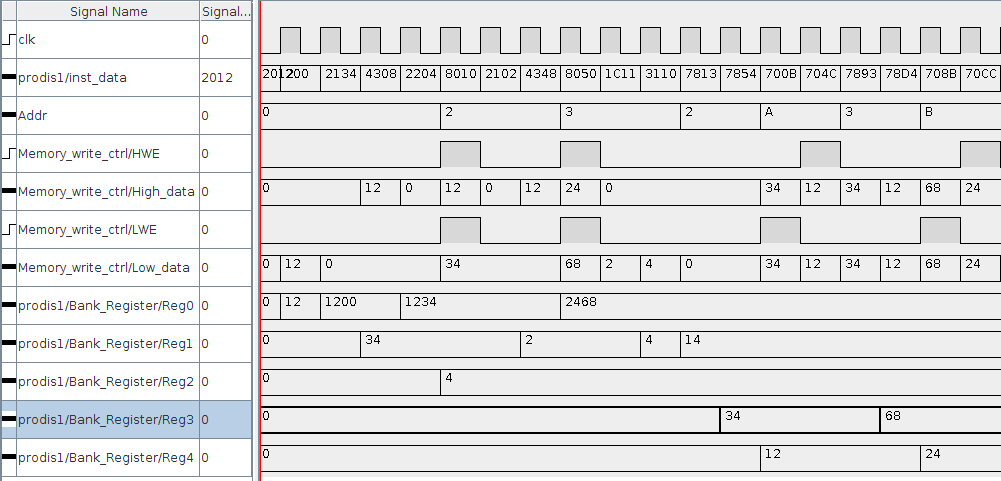
\includegraphics[width=15.8cm]{img_chrono3.png}

\subsection{Utilisation de la Pile}

Pour la deuxième étape, un code nous est fournit. Toutefois, ce code ne peut pas fonctionner. En effet, le code contient des appels de fonctions imbriqués. Lors de l'exécution d'une instruction de saut, le $Link\ Register$ est utilisé pour enregistrer l'adresse courante du PC afin de revenir au bon endroit une fois le saut terminé. Mais dans le cas où il y a plus d'un saut imbriqué, le seul moyen de pouvoir revenir en arrière, est de sauvegarder le $Link\ Register$ en mémoire.

Nous utilisons donc une partie de la mémoire comme Pile descendante pour enregistrer ces adresses. Au début de notre programme, nous initialisons le $stack\ pointer$ (r5) avec 0xfe qui est une adresse qui se trouve donc dans une partie non utilisée de la mémoire d'instruction. Ensuite, nous avons modifié le code comme suit:

A chaque fois qu'un branchement se fait vers une fonction, directement après nous enregistrons le $Link\ Register$ dans la mémoire à l'adresse contenue dans le $stack\ pointer$, et nous décrémentons immédiatement de 2 celui-ci (post-décrémentation), car c'est une pile descendante.

A chaque fin de fonction, juste avant de charger le $Link\ Register$ dans le PC, nous incrémentons de 2 le $stack\ pointer$ (pré-incrémentation) et nous chargeons l'adresse présente en mémoire, dans le $Link\ Register$.

Grâce à cette méthode, nous pouvons enregistrer beaucoup de sauts imbriqués. Le nombre dépend uniquement de la taille de la pile que nous avons à notre disposition.

\subsection{Instruction display}

Dans cette dernière partie du laboratoire, nous avons dû intégrer la gestion d'une nouvelle instruction, DISP. Cette instruction pourra afficher des pixels sur une matrice à led. Elle est utilisée avec un $.short$ car ce n'est pas une instruction officielle ARM. la syntaxe de cette instruction est la suivante: les 8 premiers bits sont fixes (0xDF) et ce sont eux que nous devons ajouter la reconnaissance dans le bloc $Decode$. Les 8 suivants sont partagés entre une valeur immédiate (5 bits) et un numéro de registre (3 bits).

Nous avons choisi de mettre le numéro de colonne de notre matrice dans la valeur immédiate, et la valeur contenue dans le registre contiendra les informations à afficher sur cette colonne. Par exemple, $.short\ 0xDF00$ affichera sur la colonne 0 le contenu de r0.

Pour commencer, nous avons ajouté au $Control\ Unit$ du bloc $Decode$ une détection de la valeur 0xdf sur les 8 premiers bits de l'instruction. Ce bit $disp\_enable$ nous permet d'effectuer plusieurs choses importantes:

D'une part, il sert de commande à un mux qui contrôle la valeur immédiate sur 5 bits. en effet, lors des instruction habituelles, la valeur immédiate sur 5 bits ne se situe pas aux bits 7-3 de l'instruction, hors c'est notre cas ici.

D'autre part, Il averti un nouveau bloc, le $Display\ Memory$ que l'écriture est active. Ce bloc contient les registres qui mémorisent les pixels des 8 colonnes de notre matrice.

Enfin, le $disp\_enable$ est utile à un autre endroit dans le bloc $Decode$. Il va commander un mux qui sélectionne le registre "actif" dans la banque de registre. Cette action est absolument nécessaire, car sinon le dernier registre qui a été initialisé se retrouve en sortie de la banque de registre, et cela a une conséquence non-négligeable sur les opérations à effectuer dans le bloc $Execute$.

En effet, dans le bloc $Execute$, le seul moyen de bypasser l'alu avec la valeur immed\_5, est d'ajouter cette valeur à un registre qui contient 0. C'est pour cela qu'au début de notre programme nous mettons le registre r0 à 0, et nous nous assurons que c'est ce registre qui est sélectionné à la sortie de la banque de registre lors d'une instruction DISP.

Une autre possibilité aurait été de modifier complètement le bloc $Execute$ pour qu'il puisse faire un bypass de la valeur immed\_5.

Quoi qu'il en soit, notre affichage à led fonctionne parfaitement.

\section{Conclusion}

Ces parties $Execute$ et $Memory\ Access$ terminent l'architecture basique de ce processeur Prodis et nous pouvons comprendre l'utilité de chacun de ces blocs. Du décodage d'instruction, aux accès mémoire, en passant par l'exécution des opérations élémentaires, nous avons à peu près fait le tour de toutes les opérations effectuée dans notre processeur. Une étape néanmoins très importante, l'architecture en pipeline, se trouvera dans le prochain laboratoire.

\end{document}